%!TEX root=../../root.tex


\section{Lezione 5}
\subsection{$\varepsilon$-mossa}
Introduciamo una mossa che permette la transizione di stato senza lettura di input. Non sempre la presenza della $\varepsilon$-mossa implica non determinismo.\newline
Ad esempio volendo costruire un automa che arrivato allo stato finale torni allo stato iniziale possiamo usare tale mossa senza creare non determinismo.\newline
\textbf{Esempio:}
\begin{figure}[H]
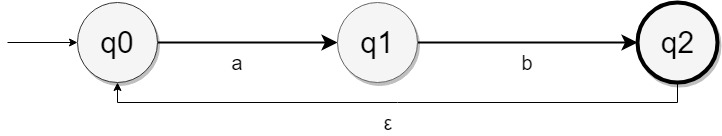
\includegraphics[scale=0.5]{l5_1}
\end{figure}
\subsection{Definizione formale di $NFA_{\varepsilon}$}
Ci\`o che cambia negli $NFA_{\varepsilon}$ \`e l'alfabeto di input, a $\Sigma$ viene aggiunta $\varepsilon$ che in questo caso rappresenta l'assenza di input. Quindi un $NFA_{\varepsilon}$ \`e una quintupla cos\`i definita:
\[
	A = (Q, \Sigma_{\varepsilon}, \lambda, q_0, F)
\]
Dove:
\[
	\Sigma_{\varepsilon} = \Sigma \cup \{\varepsilon\}
\]
\[
	\delta : Q \times \Sigma_{\varepsilon} \to {\cal P} (Q)
\]
Cambiando la definizione di $\delta$ dobbiamo ridefinire anche la funzione $delta^{\star}$:
\[
	\delta^{\star} (q, \varepsilon) = {q} \cup \delta(q, \varepsilon) 
\]
\[
	\delta^{\star} (q, xa) = \delta(\delta^{\star} (q, x), a)
\]
\textbf{Esempio:}
\begin{figure}[H]
	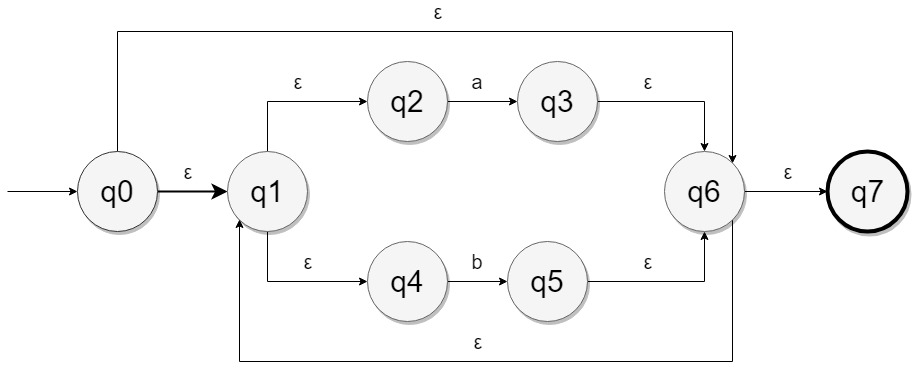
\includegraphics[scale=0.5]{l5_2}
\end{figure}

\subsection{Da $NFA_{\varepsilon}$ a $DFA$}
\subparagraph{Chiusura rispetto alla $\varepsilon$-mossa}

$\varepsilon - C(q)$ = insieme degli stati raggiungibili da q eseguendo solo $\varepsilon$ mosse.

Definiamo la chiusura di un insieme $X$ di stati rispetto alla $\varepsilon$-mossa come l'insieme degli stati raggiungibili con un numero arbitrario di $\varepsilon$ mosse da almeno uno stato nell'insieme $X$. Pi\`u formalmente:
\[
	\varepsilon-C(X) = \bigcup_{q \in X} \varepsilon-C(q)
\]

\subparagraph{Algoritmo}
\begin{description}
	\item \emph{Input:} $A = (Q, \Sigma_{\varepsilon}, \delta, q_0, F) \in NFA$
	\item \emph{Output:} $A' = (Q', \Sigma, \delta', q'_0, F') \in DFA$ tale che $L(A) = L(A')$
	\item \emph{Algoritmo:}
		\begin{enumerate}[label*=\arabic*.]
			\item Poni $Q' = \varepsilon-C(q_0)$
			\item Ripeti finch\`e in $Q'$ ci sono stati non marcati
				\begin{enumerate}[label*=\arabic*.]
					\item Prendi un elemento non marcato $X \in Q'$
					\item $\forall a \in \Sigma$
						\begin{enumerate}[label*=\arabic*.]
							\item $Y_a = \bigcup_{p \in X} \delta(p,a) \cup \varepsilon - C(p)$
							\item $\delta'(X,a) = Y_a$
							\item $Y_a \notin Q' \Rightarrow$ aggiungi $Y_a$, non marcato, in $Q'$  						
						\end{enumerate}
			\item $\forall X \in {\cal P}(Q) - Q' \Rightarrow \delta'(X, a) = \emptyset$ $ \forall a \in \Sigma$. Questo serve per rendere $\delta$ completo.
			\item Poni $q'_0 = \varepsilon - C(q_0)$ e $F' = \{Y \in Q' | Y \cap F \neq \emptyset\}$
				\end{enumerate}
		\end{enumerate}
\end{description}
\textbf{Esempio:} Il DFA che segue \`e il risultato dell'applicazione dell'algoritmo sull'NFA dell'esempio precedente. \newline
\begin{figure}[H]
	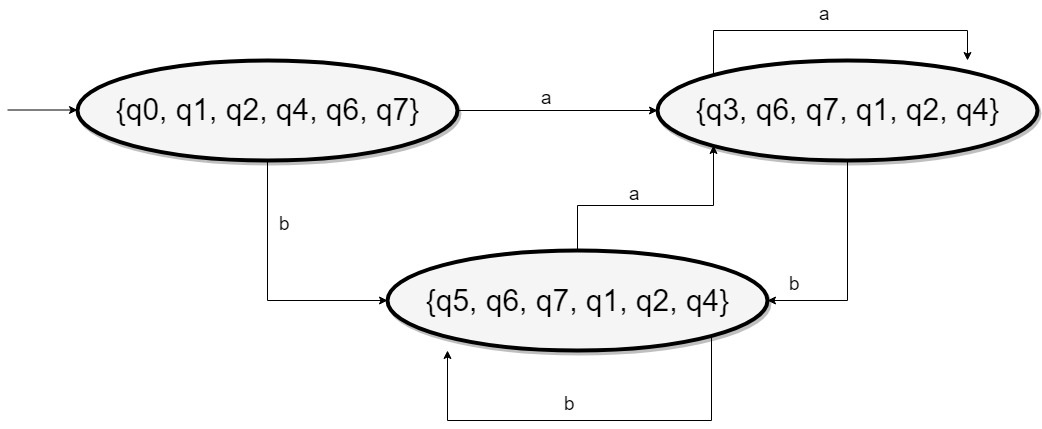
\includegraphics[scale=0.35]{l5_3}
\end{figure}
\subsection{Automa prodotto}
Siano $A_1$ e $A_2$ due automi cos\`i definiti:\newline
$A_1 = (Q_1, \Sigma, \delta_1, q^1_0,F_1)$ tale che $L = L(A_1)$ \newline $A_2 = (Q_2, \Sigma, \delta_2, q^2_0,F_2)$ tale che $L' = L(A_2)$  \newline
e che valga $Q_1 \cap Q_2 = \emptyset$. \newline
L'automa prodotto \`e $A = (Q_1 \cup Q_2, \Sigma_{\varepsilon}, \delta, q^1_0, F_2)$ con $\delta$ definita come segue:
\[
	A = (Q_1 \cup Q_2, \Sigma_{\varepsilon}, \delta, q_0^1, F_2)
\]
Dove:
\[
	\delta(q,a) = \delta_1(q,a) \forall  q \in Q_1-F_1, \forall a \in \Sigma_{\varepsilon}
\]
\[
	\delta(q,a) = \delta_1(q,a) \forall  q \in F_1, \forall a \in \Sigma
\]
\[
	\delta(q,\varepsilon) = \delta_1(q,\varepsilon) \cup {q_0^2} \forall  q \in F_1
\]
\[
	\delta(q,a) = \delta_2(q,a) \forall  q \in Q_2, \forall a \in \Sigma
\]

%\begin{figure}
	%\includegraphics[scale=0.5]{}
%\end{figure}

\subsection{Automa chiusura a stella di Kleene}
Siano $A'$ un automa cos\`i definito:\newline
$A' = (Q, \Sigma, \delta', q_0,F)$ tale che $L = L(A')$ \newline
L'automa che accetta $L^{\star}$ \`e definito come segue:
\[
	A = (Q \cup \{p_0\}, \Sigma_{\varepsilon}, \delta, q_0, F \cup \{p_0\})
\]
Dove:
\[
	p_0 \notin Q
\]
\[
	\delta(q,a) = \delta'(q,a) \forall  q \in Q-F, \forall a \in \Sigma
\]
\[
	\delta(p_0,\varepsilon) =  \{q_0\}
\]
\[
	\delta(q,a) = \delta'(q,a) \forall  q \in F_1, \forall a \in \Sigma
\]
\[
	\delta(q,\varepsilon) = \delta'(q,\varepsilon) \cup {q_0} \forall  q \in F_1
\]
\begin{figure}[H]
	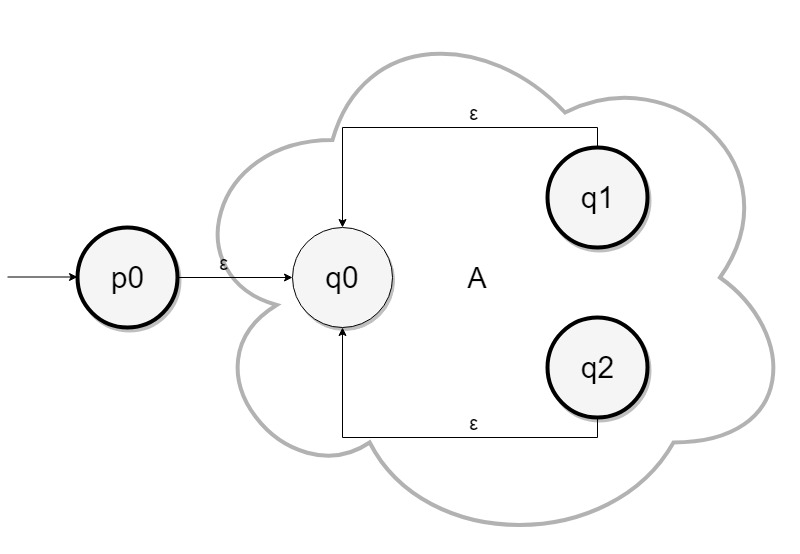
\includegraphics[scale=0.35]{l5_5}
\end{figure}
\textbf{Esempio:} Automa che riconosce il linguaggio $L = \{L^{\star}\}$
\begin{figure}[H]
	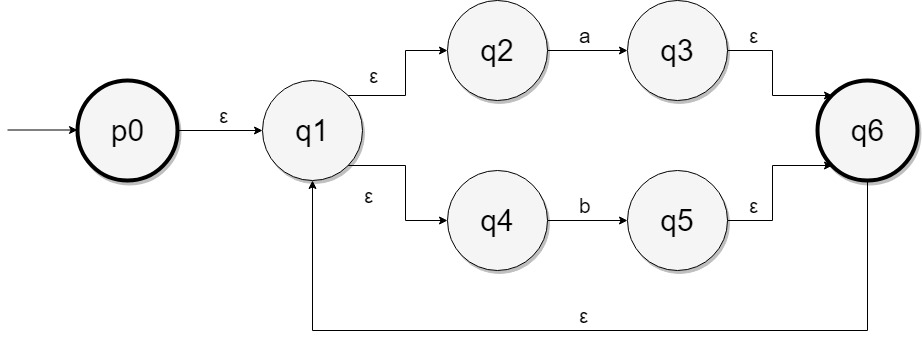
\includegraphics[scale=0.4]{l5_6}
\end{figure}

\subsection{Automa complemento}
Per ottenere l'automa complemento di un $NFA$ bisogna prima passare al $DFA$ equivalente e poi effettuare il complemento su di esso.

